\chapter{Motivation}
\label{motiv}
In the institute of reliable Embedded Systems and Communication Electronics
(ivESK) is a project named \embtls which has the goal to use the TLS protocol
(see section \ref{tls_proto}) in embedded systems.

\begin{figure}[!ht]
\centering
%\frame{
% trim: left, bottom, right, up
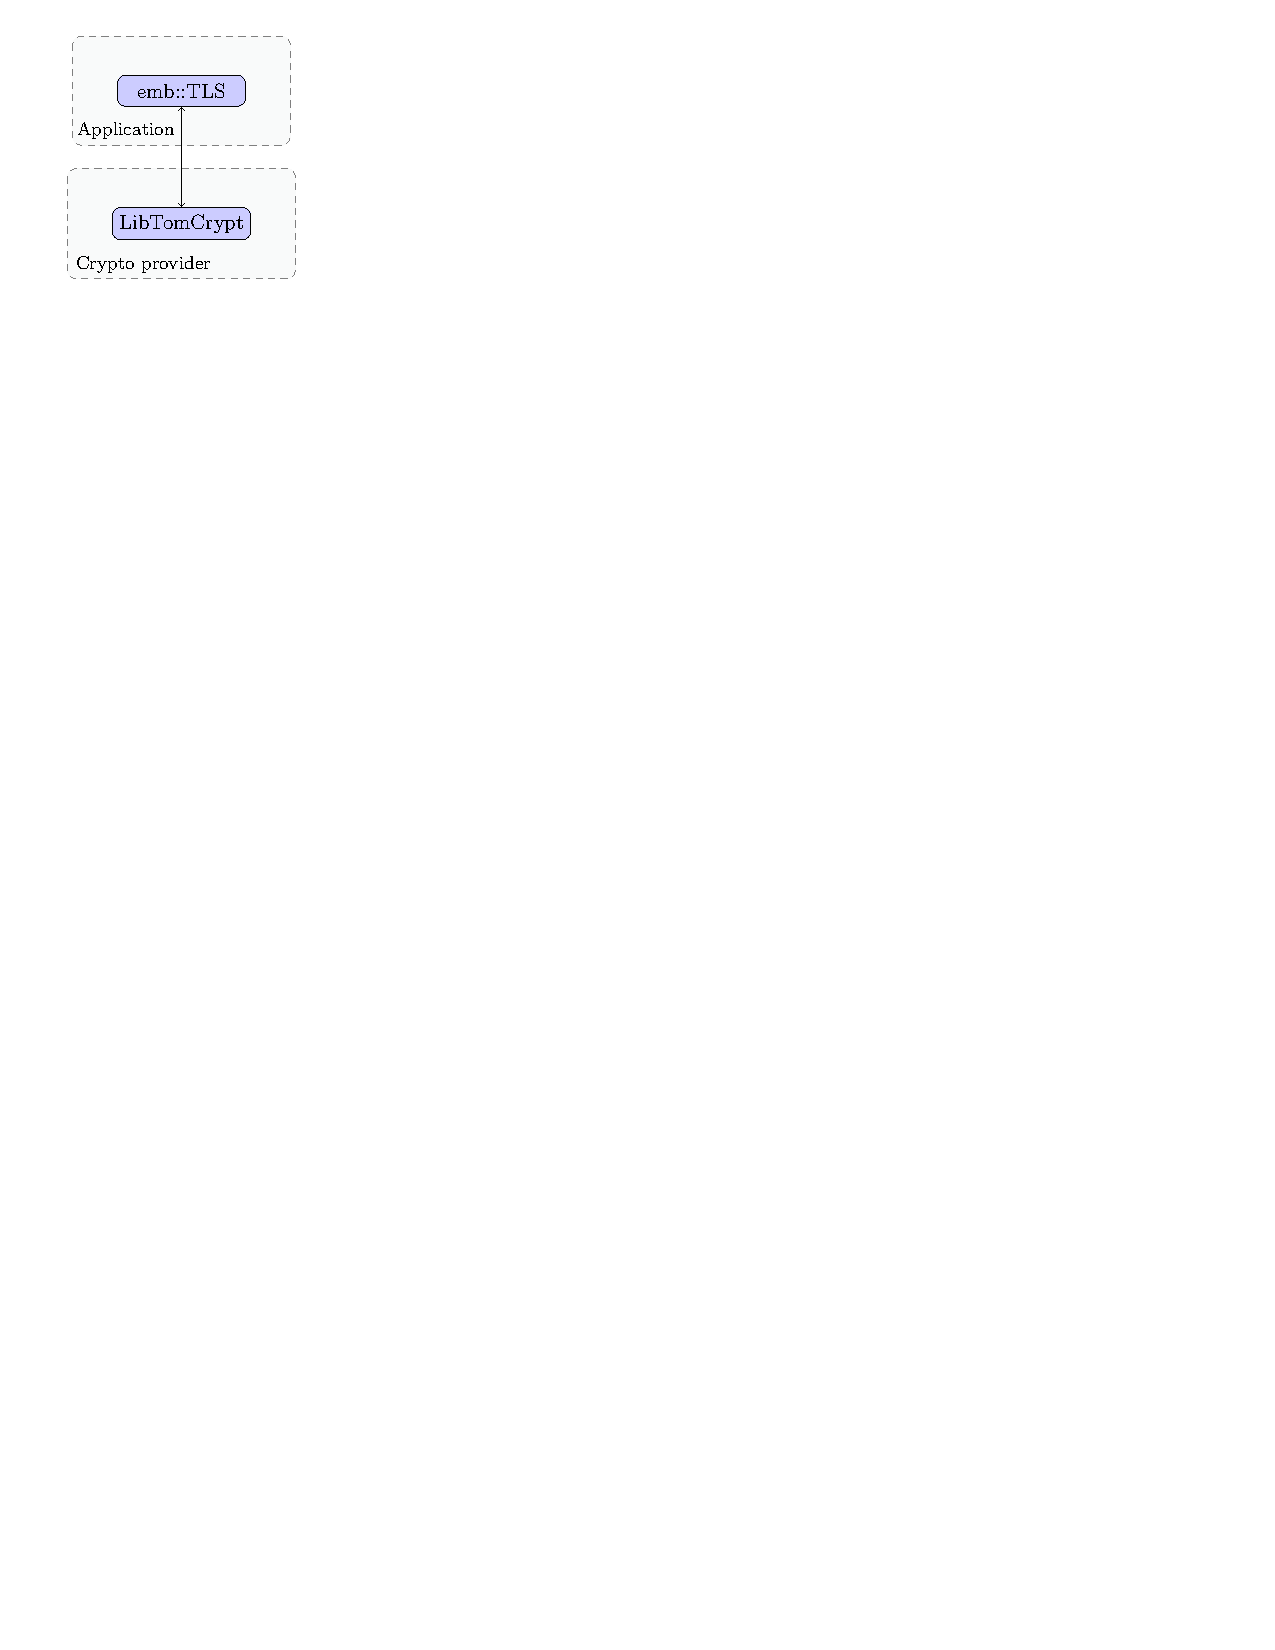
\includegraphics[trim=0cm 23.25cm 15.25cm 0cm,
height=6.5cm]{figures/intro_embtls.pdf}
\caption{\embtls's project}
\label{fig:motiv_embtls}
%}

\end{figure}

The project, \embtls, uses a library, named \tomcrypt, which is an open-source 
cryptographic software library and is used for the calculation needed by the
cryptographic algorithms (see figure \ref{fig:motiv_embtls}).
The institute wants, however, to have the possibility to use other providers,
needed for the calculation of the cryptographic algorithms, to make comparison
between them.
Unfortunately, to change the provider, the application, \embtls, has to be
completely changed, which will take a long time, because the project is quick
long.
That's why the use of an interface, as API, will be very useful.
The interface will have a base of cryptography, with the main
cryptographic algorithms, defined in the chapter \ref{intro}.
It will be implemented in the application, i.e \embtls, and will use a
cryptographic provider for the calculation (see figure \ref{fig:motiv_gci}).
The most important advantage of the use of the interface is when the change of a
provider has to be done, without the interface, the functions of the provider
are oft called several times in the application, and also has to be changed each time.
With the interface, a function of it can be called several times in the
application, but that has no effect if the provider changes. The
change is only done in the interface part (see figure \ref{fig:motiv_gci}).
That will, also, take less time to change a provider by using the interface.
 

\begin{figure}[!ht]
\centering
%\frame{
% trim: left, bottom, right, up
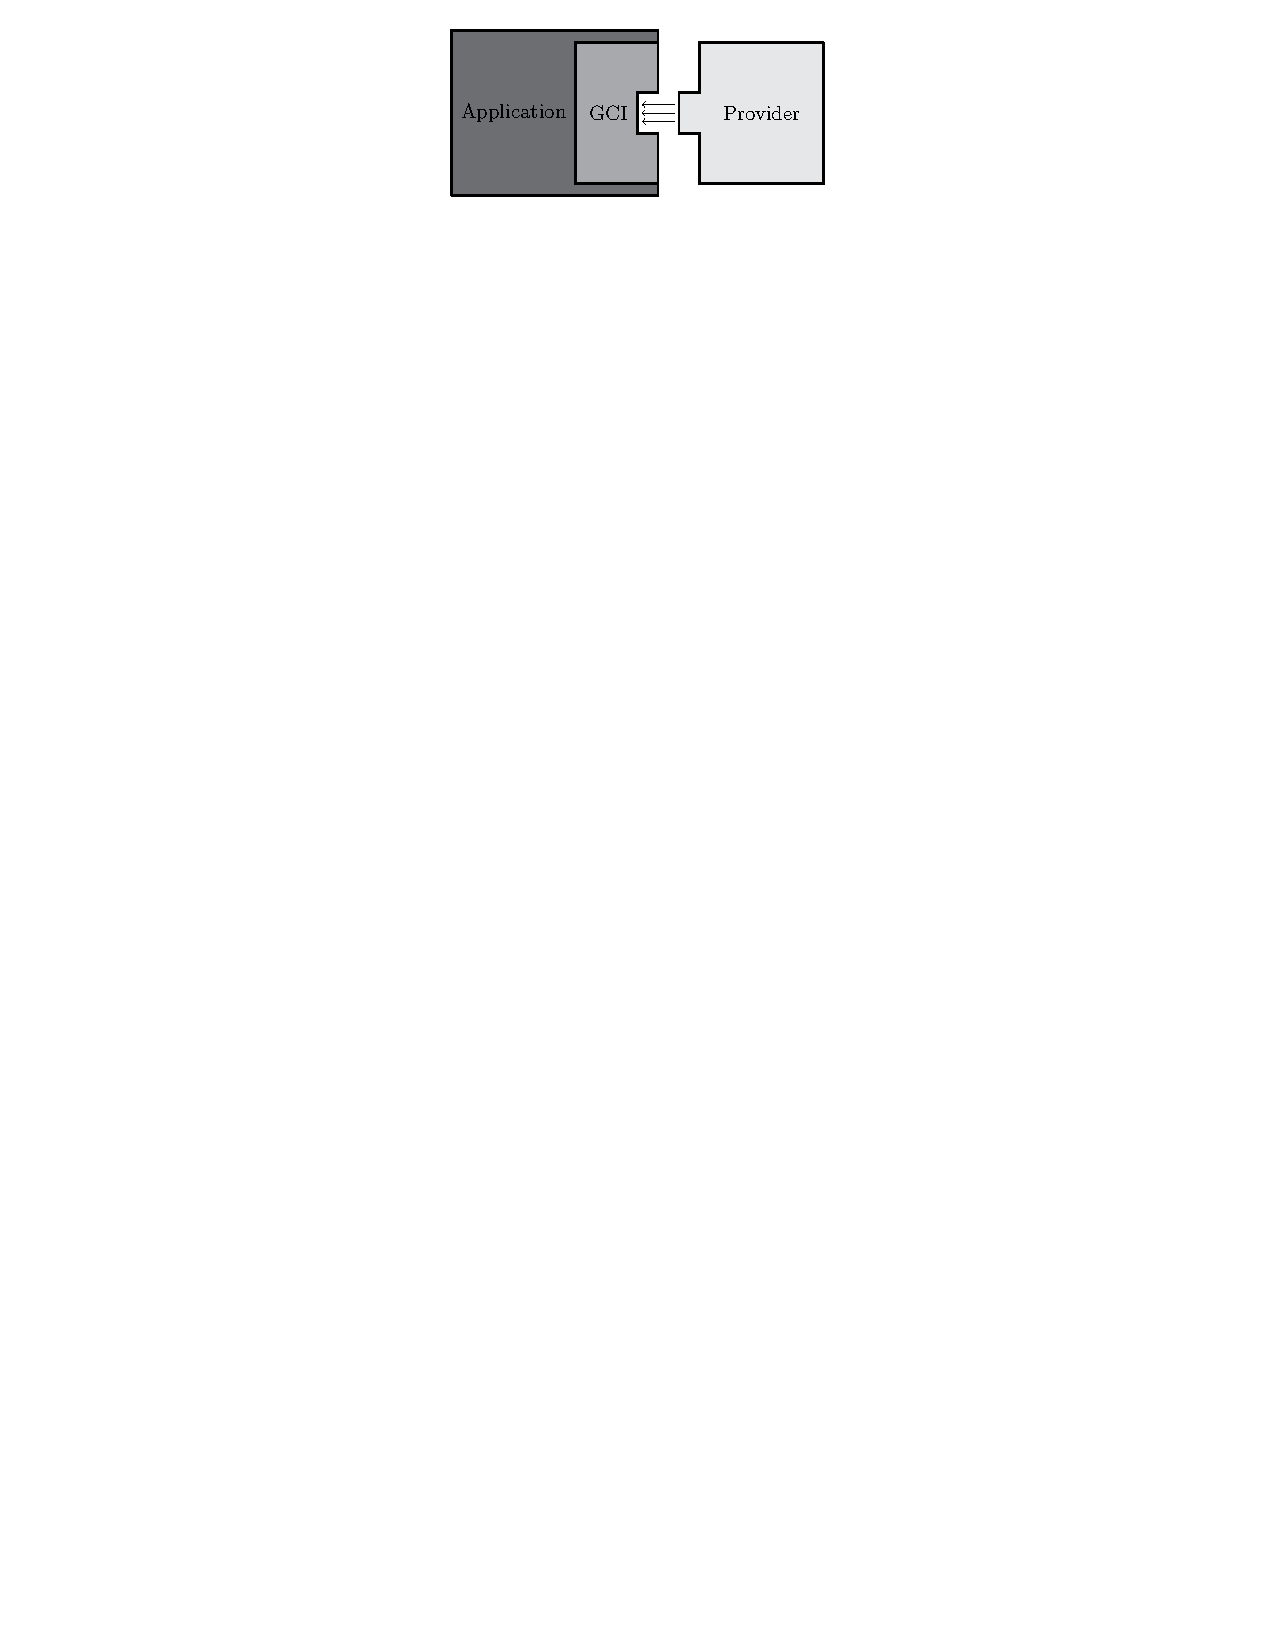
\includegraphics[trim=4.5cm 24.5cm 2cm 0cm, height=4.5cm]{figures/intro_gci.pdf}
\caption{Goal of the new implementation}
\label{fig:motiv_gci}
%}
\end{figure}

The goal of this thesis is therefore to design this interface to have a
base of the main cryptographic algorithms. The interface has to be as
generic as possible to use different kinds of cryptographic providers, which can
be an open-source cryptographic software library (i.e \tomcrypt
\cite{doc:tomcrypt}) or a hardware-based cryptographic module (i.e \vaultic
\cite{doc:vault}), and to be used in different applications.
The institute wants to use hardware-based cryptographic module with one of its
particularities of key management.
The interface shall have a key management too, so it can be possible to use it
from the hardware-based cryptographic module.
When a cryptographic algorithm of the interface is used, it has to be
possible to configure it. The behavior of the algorithm should only be assigned
by the parameters coming from the configuration. No hidden states shall be used
in the interface's function, meaning that all parameters
written in input of the function, as configuration, will be used for the
cryptographic algorithm and nothing else.

